\section{Paper 8}
\subsection{\emph{"Visual Object Tracking via Multi-Stream Deep Similarity Learning Networks"}}

\begin{frame}{INTRODUCTION}
    The goal of visual tracking systems is to be able to obtain the position of 
    the tracked target even in subsequent frames. The problems to be solved 
    are those of occlusion, background clutter, illumination variations, 
    deformation etc. The following paper uses a model that compares 
    similarities and is trained offline in order to predict the patch present in 
    the next frame. The method, thanks to the use of the relative distance, 
    is robust in the presence of phenomena that introduce the so called 
    \emph{distractors}.
\end{frame}

\begin{frame}{RELATED WORK}
    Some methods train a CNN offline while the test is done online. Unfortunately, 
    these models are not fast. Other models instead if they fail a first 
    time, then they will always fail until the target returns to the search region. 
    Other methods \footfullcite{0893551129} \footfullcite{0893551134} search for the target template in subsequent frames 
    in the same position, obtaining better performance than methods based on 
    similarity but nevertheless are not robust to distracting elements. The proposed 
    method instead takes into account both the \emph{background patches} and 
    the \emph{target template patches} in order to make comparisons on similarities.
\end{frame}

\begin{frame}{METHODS - EMDSLT Architecture}
    The proposed framework, called Ensemble Multi Deep Stream Similarity 
    Learnining Tracking (EMDSLT), is composed of some netwroks. Those 
    in blue are fully-convolutional networks while those in red are useful for 
    re-verification and re-detection operations, responsible for recovery from 
    failures and the template updating.
    \begin{figure}[h!]
        \centering
        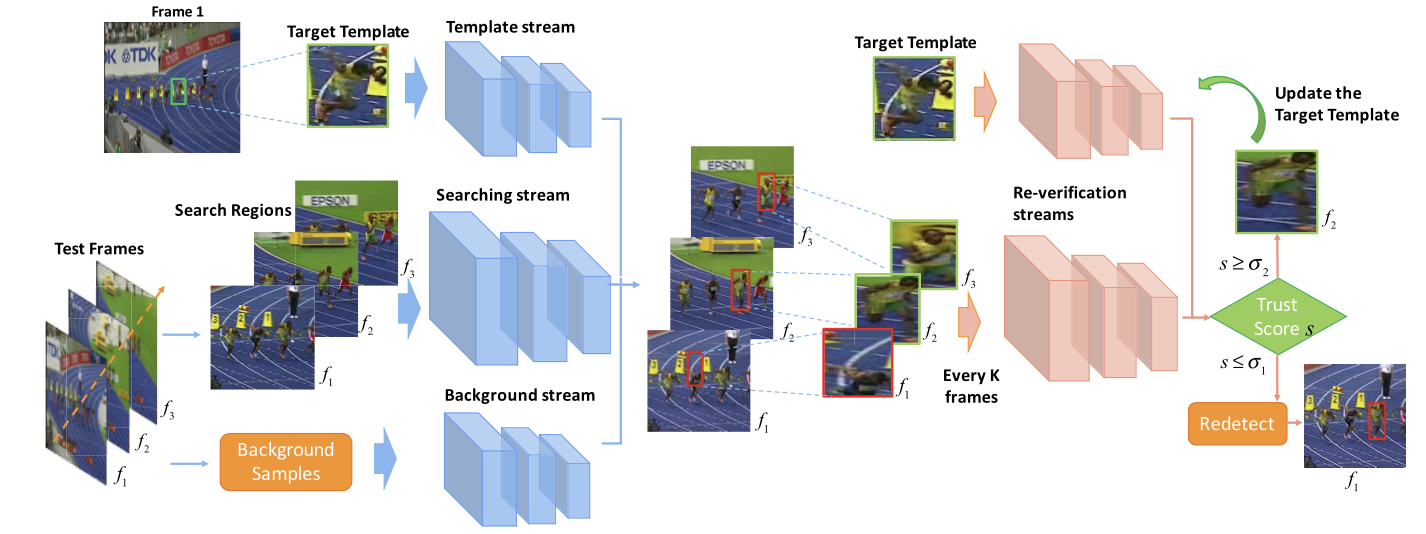
\includegraphics[width = \linewidth]{images/paper8/EMDSLT.png}
        \centering
        \caption{The EMDSLT framework.}
        \label{fig:EMDSLT}
    \end{figure}
\end{frame}

\begin{frame}{METHODS - Streams}
    The target template \emph{T}, the patches $X_i^+$ positive and the background patches $B_{i-1,j}$, are extracted from the first convolutional networks. These elements are useful for calculating the \emph{Template-Searching-Background Loss} (TSB).
    \begin{figure}[h!]
        \centering
        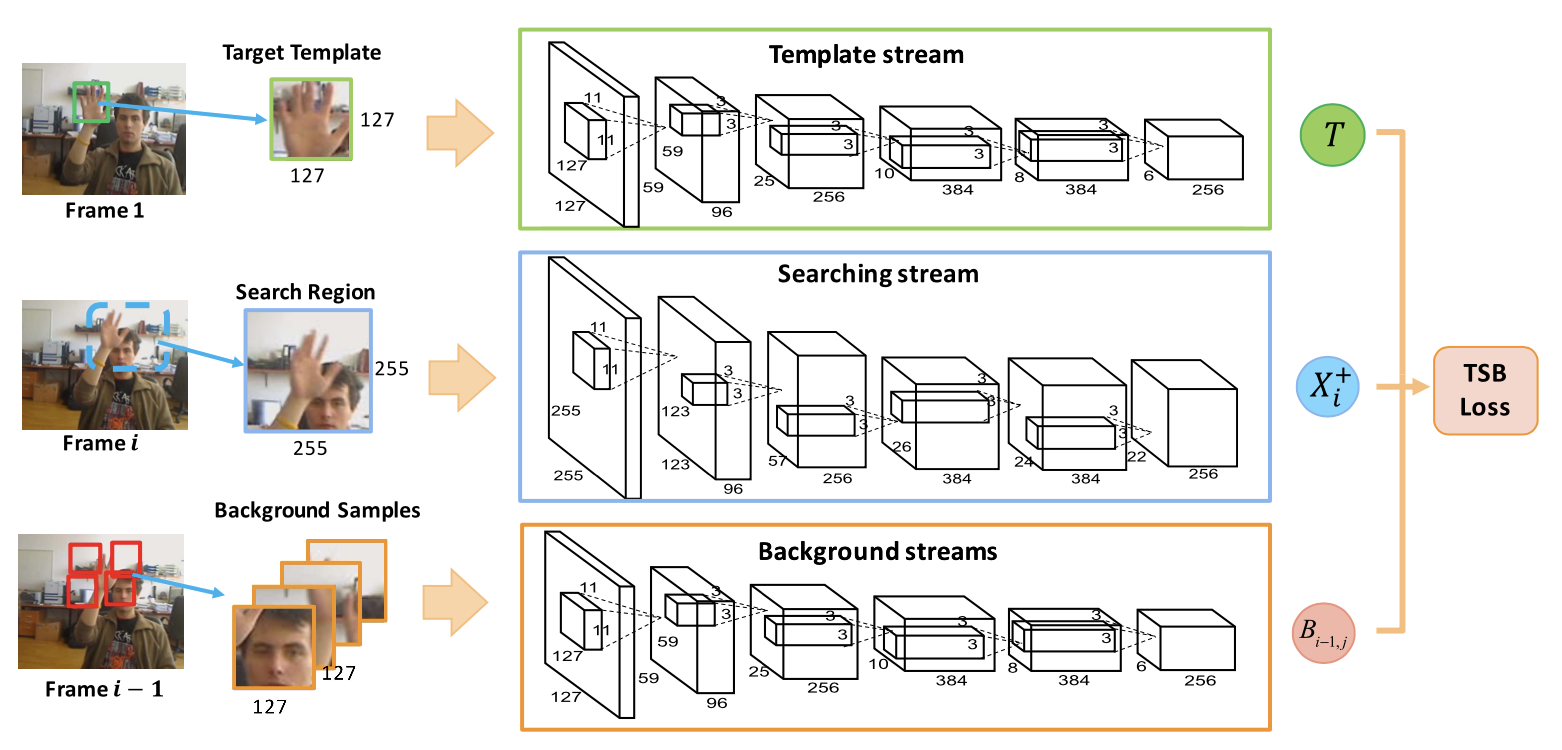
\includegraphics[width = \linewidth]{images/paper8/streams.png}
        \centering
        \caption{Multi Deep Streams}
        \label{fig:streams}
    \end{figure}
\end{frame}

\begin{frame}{METHODS - \emph{Template-Searching-Background Loss} (TSB)}
    
\end{frame}